% !TeX spellcheck = en_US
% !TeX encoding = UTF-8
\section{Replica Exchange Molecular Dynamics\label{Sec:ES:REMD}}
\subsection{Temperature-Replica Exchange Molecular Dynamics\label{Sec:ES:REMD:TREMD}}
The idea of replica exchange was proposed by Swendsen and Wang.\cite{SwendsenPRL1986} Temperature replica exchange molecular dynamics (T-REMD) is one class of parallel tempering methods developed by Hansmann, Okamoto and Sugita\cite{HansmannJCC1993,HansmannCPL1997,SugitaCPL1999} based on many ideas in a category of methods called \textit{generalized-ensemble algorithm}. It is an extension of the well-known simulated annealing method. The basic idea of REMD is schematically summarized in Fig.~\ref{Fig:ES:REMD}. In REMD, the system is replicated into $\mathbf{M}$ \textit{non-interacting} copies (replicas). Each replica is coupled to a bath at temperature $T_m$, $(m=1,\dots,M)$. At a certain time, the system is at state $X$, which can be denoted as $X=\left(x_1^{[i(1)]},\dots,x_M^{[i(M)]}\right)=\left(x_{m(1)}^{[1]},\dots,x_{m(M)}^{[M]}\right)$. Here, we used $i$ and $m$ to label the replica and the temperature respectively. Because the replicas are non-interacting, the weight-factor for a state $X$ in this generalized ensemble is a direct product of the Boltzmann factors for each replica, i.e.
\begin{equation}
	W_{REM}(X)=\prod\limits_{m=1}^M\exp{\left(-\beta_m H\left(q^{[i(m)]},p^{[i(m)]}\right)\right)}=\prod\limits_{i=1}^M \exp{\left(-\beta_{m(i)}H\left(q^{[i]},p^{[i]}\right)\right)}\textsl{}
\end{equation}

\begin{figure}[htbp]
	\centering
	%	\resizebox{2cm}{!}{
	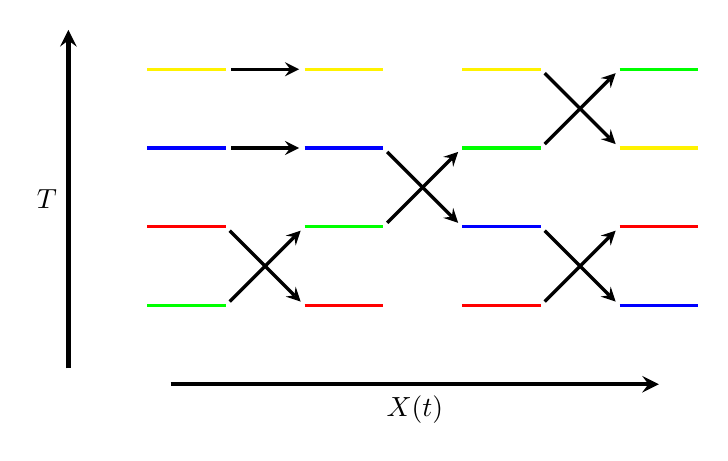
\begin{tikzpicture}
	    \draw[ultra thick,->,>=stealth] (1.3,0) -- (7.5,0) node[midway,below]{$X(t)$};
	    \draw[ultra thick,->,>=stealth] (0,0.2) -- (0,4.5) node[midway,left]{$T$};
	    
        \draw[very thick,green] (1,1) -- (2,1);
        \draw[very thick,red] (1,2) -- (2,2);
        \draw[very thick,blue] (1,3) -- (2,3);
        \draw[very thick,yellow] (1,4) -- (2,4);
        
        \draw[very thick,->,shorten >=2pt,shorten <=2pt,>=stealth] (2,1) -- (3,2);
        \draw[very thick,->,shorten >=2pt,shorten <=2pt,>=stealth] (2,2) -- (3,1);
        \draw[very thick,->,shorten >=2pt,shorten <=2pt,>=stealth] (2,3) -- (3,3);
        \draw[very thick,->,shorten >=2pt,shorten <=2pt,>=stealth] (2,4) -- (3,4);
        
        \draw[very thick,red] (3,1) -- (4,1);
        \draw[very thick,green] (3,2) -- (4,2);
        \draw[very thick,blue] (3,3) -- (4,3);
        \draw[very thick,yellow] (3,4) -- (4,4);
        
        \draw[very thick,->,shorten >=2pt,shorten <=2pt,>=stealth] (4,2) -- (5,3);
        \draw[very thick,->,shorten >=2pt,shorten <=2pt,>=stealth] (4,3) -- (5,2);
        
        \draw[very thick,red] (5,1) -- (6,1);
        \draw[very thick,blue] (5,2) -- (6,2);
        \draw[very thick,green] (5,3) -- (6,3);
        \draw[very thick,yellow] (5,4) -- (6,4);
        
        \draw[very thick,->,shorten >=2pt,shorten <=2pt,>=stealth] (6,1) -- (7,2);
        \draw[very thick,->,shorten >=2pt,shorten <=2pt,>=stealth] (6,2) -- (7,1);
        \draw[very thick,->,shorten >=2pt,shorten <=2pt,>=stealth] (6,3) -- (7,4);
        \draw[very thick,->,shorten >=2pt,shorten <=2pt,>=stealth] (6,4) -- (7,3);
        
        \draw[very thick,blue] (7,1) -- (8,1);
        \draw[very thick,red] (7,2) -- (8,2);
        \draw[very thick,yellow] (7,3) -- (8,3);
        \draw[very thick,green] (7,4) -- (8,4);        
	\end{tikzpicture}
	%	}
	\caption{A schematic representation of replica exchange molecular dynamics.}\label{Fig:ES:REMD}
\end{figure}

%\begin{figure}[htbp]
%    \centering
%	\includegraphics[width=0.6\textwidth]{figures/REMD.pdf}\\
%	\caption{A schematic representation of replica exchange molecular dynamics.}\label{Fig:ES:REMD}
%\end{figure}

Now, we exchange the temperatures of a pair of replicas
\begin{equation}
	\left\{ 
	\begin{array}{rcll} 
		x_m^{[i]}\equiv& \left(q^{[i]},p^{[i]}\right)_m \Rightarrow x_n^{[i]^\prime}&\equiv \left(q^{[i]},p^{[i]^\prime}\right)_n&\\ 
		&&&,\\
		x_n^{[j]}\equiv& \left(q^{[j]},p^{[j]}\right)_n \Rightarrow x_m^{[j]^\prime}&\equiv \left(q^{[j]},p^{[j]^\prime}\right)_m&\\  
	\end{array} 
	\right. 
\end{equation}
where
\begin{equation}
	\left\{ 
	\begin{array}{rl} 
		p^{[i]^\prime}\equiv \sqrt{\frac{T_n}{T_m}} p^{[i]}&\\ 
		&.\\
		p^{[j]^\prime}\equiv \sqrt{\frac{T_m}{T_n}} p^{[j]}&\\  
	\end{array} 
	\right. 
\end{equation}
The exchange rule is not trivial. In order for this exchange process to converge towards an equilibrium distribution, it is sufficient to impose the detailed balance condition on the transition probability $w(X\rightarrow X^\prime)$:
\begin{equation}
	W_{REM}(X)w(X\rightarrow X^\prime) = W_{REM}(X^\prime)w(X^\prime\rightarrow X).
\end{equation}
Then we have
\begin{align}
	&\frac{w\left(X\rightarrow X^\prime\right)}{w\left(X^\prime\rightarrow X\right)}\notag\\
	=&\frac{W_{REM}(X^\prime)}{W_{REM}(X)}\notag\\
	   =&\frac{\exp{\left(-\beta_m H\left(q^{[j]},p^{[j]^\prime}\right)\right)}\exp{\left(-\beta_n H\left(q^{[i]},p^{[i]^\prime}\right)\right)}}{\exp{\left(-\beta_m H\left(q^{[i]},p^{[i]^{ }}\right)\right)}\exp{\left(-\beta_n H\left(q^{[j]},p^{[j]^{ }}\right)\right)}}\notag\\
	   =&\frac{\exp{\left\{-\beta_m\left[K\left(p^{[j]^\prime}\right)+U\left(q^{[j]}\right)\right]-\beta_n\left[K\left(p^{[i]^\prime}\right)+U\left(q^{[i]}\right)\right]\notag\right\}}}
	   {\exp{\left\{-\beta_m\left[K\left(p^{[i]}\right)+U\left(q^{[i]}\right)\right]-\beta_n\left[K\left(p^{[j]}\right)+U\left(q^{[j]}\right)\right]\notag\right\}}}\notag\\
	   =&\frac{\exp{\left\{-\beta_m\left[\frac{T_m}{T_n}K\left(p^{[j]}\right)+U\left(q^{[j]}\right)\right]-\beta_n\left[\frac{T_n}{T_m}K\left(p^{[i]}\right)+U\left(q^{[i]}\right)\right]\notag\right\}}}
	   {\exp{\left\{-\beta_m\left[K\left(p^{[i]}\right)+U\left(q^{[i]}\right)\right]-\beta_n\left[K\left(p^{[j]}\right)+U\left(q^{[j]}\right)\right]\notag\right\}}}\notag\\
	   =&\dfrac{\exp{\left\{-\beta_n K\left(p^{[j]}\right)-\beta_m K\left(p^{[i]}\right)\right\}}}{\exp{\left\{-\beta_m K\left(p^{[i]}\right)-\beta_n K\left(p^{[j]}\right)\right\}}} \dfrac{\exp{\left\{-\beta_m U\left(q^{[j]}\right)-\beta_n U\left(q^{[i]}\right)\right\}}}{\exp{\left\{-\beta_m U\left(q^{[i]}\right)-\beta_n U\left(q^{[j]}\right)\right\}}}\notag\\
	   =&\exp{\left\{-\Delta\right\}}.
\end{align}
where $\Delta = \left[\beta_n-\beta_m\right]\left[U\left(q^{[i]}\right)-U\left(q^{[j]}\right)\right]$. It can be seen that the kinetic energy terms are fully canceled out.
This can be satisfied by the usual Metropolis criterion:
\begin{equation}
	w\left(X\rightarrow X^\prime\right)\equiv w\left(x_m^{[i]}\, \bigg\rvert\, x_n^{[j]}\right)= 
	\left\{ 
	\begin{array}{ll} 
		1, & \text{if } \Delta \leq 0\\ 
		\exp{(-\Delta)}, & \text{if } \Delta >0\\  
	\end{array} 
	\right. 
\end{equation}

The high-temperature replicas and the low-temperature replicas work in a collaborative way, in which the former explore phase space while the latter exploit phase space around local minima. The convergence rate is highly correlated to the acceptance ratio of exchange between neighboring replicas.  Kofke found that, for systems with Gaussian energy distributions, the average acceptance ratio is given by\cite{KofkeJCP2002,KofkeJCP2004a,KofkeJCP2004b}
\begin{equation}
	\left<\bar{p}_{acc}\right>=\erfc\left[\left(\frac{1}{2}C_v\right)^{1/2}\frac{1-\beta_j/\beta_i}{(1+(\beta_j/\beta_i)^2)^{1/2}}\right],
\end{equation}
where $C_v$ is the heat capacity at constant volume and is assumed to be constant in the temperature range between $\beta_i$ and $\beta_j$.
After long time simulations, all the replicas have arrived at a global equilibrium. In order to calculate the free energy or the ensemble average of an operator $\hat A$ at $T_m$, we can extract all the snapshots that have a temperature $T_m$ from $M$ trajectories, if this temperature was among the $M$ chosen temperatures. However, the optimal way is to use Weighted Histogram Analysis Method in Section~\ref{Sec:FEM:WHAM} or the Multistate Bennett Acceptance Ratio method in Section~\ref{Sec:FEM:MBAR}.  

In the above derivation, it only considers exchanges between neighboring states. However, a global permutation is also possible, and sometimes it may improve sampling efficiency.\cite{ChoderaJCP2011} REMD has been extended to Tsallis statistics\cite{WhitfieldPA2002}.

\subsection{Hamiltonian-Replica Exchange Molecular Dynamics\label{Sec:ES:REMD:HREMD}}
Another type of REMD simulation is called Hamiltonian replica exchange molecular dynamics (H-REMD), in which each replicas has its own Hamiltonian, but is coupled to the same temperature.\cite{JangPRL2003} One example is the H-REMD simulation for a torsional angle. The $m$th replica has a torsional energy term of 
\begin{equation}
	H_m(\phi)=\lambda(m)\sum_n\left(V_n/2\right)\left(1+\cos{\left[n\phi-\delta\right]}\right),
\end{equation}
where $\lambda$ is a control parameter. $\lambda(0)=1$ corresponds to the unbiased state and at $\lambda(M)$ (usually $\lambda(M)=0$) the torsional motion of this dihedral angle has a smaller barrier.

Another example of HREMD is pH-REMD, in which each replica is coupled with different pH of the solution. In other words, the chemical potential of hydronium in each replica is different . Therefore, the protonation states (or probability of being protonated or deprotonated) of titratable residues in each replica may differ from those in other replicas. In the simulations, the protonation states of titratable residues have their protonation states alternated according to the Metropolis criterion
\begin{equation}
	P= 
	\left\{ 
	\begin{array}{ll} 
		1, & \text{if } \Delta G_{\ce{P_{A}}\rightarrow \ce{P_{A}H^{+}}}\leq 0\\ 
		\exp{(-\beta\Delta G_{\ce{P_{A}}\rightarrow \ce{P_{A}H^{+}}})}, & \text{if }\Delta G_{\ce{P_{A}}\rightarrow \ce{P_{A}H^{+}}} >0\\  
	\end{array} 
	\right. 
\end{equation}
using Monte Carlo. The derivation of $\Delta G_{\ce{P_{A}}\rightarrow \ce{P_{A}H^{+}}}$ is shown below. 

Free energy of molecule \ce{A} in solution with a concentration $\left[\ce{A}\right]$
can be written as 
\[
\Delta G_{\ce{A}}=\Delta G_{\ce{A}}^{0}+\beta^{-1}\ln\frac{\left[\ce{A}\right]}{C_{0}},
\]
in which $\Delta G_{\ce{A}}^{0}$ is the free energy of molecule A at the standard
state $C_{0}$, i.e. 1 mol/L. The free energy change for a reaction
\begin{center}
	\schemestart \chemfig{A} + \chemfig{B} \arrow{<=>}[,0.75] \chemfig{C} \schemestop
\end{center}
%\[
%A+B\rightleftharpoons C
%\]
can be written as
\[
\Delta G=\Delta G_{\ce{C}}-\Delta G_{\ce{A}}-\Delta G_{\ce{B}}=\Delta G_{0}+\beta^{-1}\ln\frac{\left[\ce{C}\right]C_{0}}{\left[\ce{A}\right]\left[\ce{B}\right]}.
\]

At equilibrium, the free energy change is zero, we have
\begin{equation}
	\Delta G_{0}=-\beta^{-1}\ln\frac{\left[\ce{C}\right]C_{0}}{\left[\ce{A}\right]\left[\ce{B}\right]},\label{eq:FEM:REMD:standardfreeenergy}
\end{equation}
in which $\left[\ce{A}\right]\left[\ce{B}\right]/\left[\ce{C}\right]C_{0}$ is called
the dissociation constant $K_{a}$. So,

\begin{equation}
\Delta G_{0}=\beta^{-1}\ln K_{a}.
\label{eq:FEM:REMD:standardfreeenergyvsKa}
\end{equation}

Titration of a residue in a real protein can be written as
\begin{center}
	\schemestart \chemfig{P_{A}} + \chemfig{H^{+}} \arrow{<=>}[,0.75] \chemfig{P_{A}H^{+}} \schemestop
\end{center}
%\[
%P_{A}+H^{+}\rightleftharpoons P_{A}H^{+},
%\]

with 
\[
K_{a}=\frac{\left[\ce{P_{A}}\right]\left[\ce{H^{+}}\right]}{\left[\ce{P_{A}H^{+}}\right]C_{0}}
\]

The fraction of the deprotonated species is calculated as

\begin{eqnarray}
	f_{\left[\ce{P_{A}}\right]} & = & \frac{\left[\ce{P_{A}}\right]}{\left[\ce{P_{A}}\right]+\left[\ce{P_{A}H^{+}}\right]}\nonumber \\
	& = & \frac{1}{1+\frac{\left[\ce{P_{A}H^{+}}\right]}{\left[\ce{P_{A}}\right]}}\nonumber \\
	& = & \frac{1}{1+\frac{\left[\ce{P_{A}}\right]\left[\ce{H^{+}}\right]}{C_{0}K_{a}\left[\ce{P_{A}}\right]}}\nonumber \\
	& = & \frac{1}{1+\frac{1}{C_{0}K_{a}}\left[\ce{H^{+}}\right]}\nonumber \\
	& = & \frac{1}{1+\frac{1}{K_{a}}10^{-\mathrm{pH}}}\label{eq:FEM:REMD:titrationcurve}
\end{eqnarray}
We can check the asymptotic behavior of this equation. At strong
acidic condition ($\mathrm{pH}=-\infty$), $f_{\left[\ce{P_{A}}\right]}=0$, indicating that
the residue is 100 percent protonated. While at an extremely basic
condition ($\mathrm{pH}=\infty$), $f_{\left[\ce{P_{A}}\right]}=1$. This residue is 100
percent deprotonated. From the Henderson–Hasselbalch (HH) equation, 
the $\mathrm{p}K_a$ can be determined by the $\mathrm{pH}$ of the state when 
$\left[\ce{P_{A}}\right]/\left[\ce{P_{A}H^{+}}\right]=1$

\begin{align}
	\mathrm{p}K_{a}  = & -\log{K_{a}}\notag\\
	 = & -\log{\frac{\left[\ce{P_{A}}\right]}{\left[\ce{P_{A}H^{+}}\right]}}-\log{\frac{\left[\ce{H^{+}}\right]}{C_{0}}}\notag\\
	 = & -\log{\frac{\left[\ce{P_{A}}\right]}{\left[\ce{P_{A}H^{+}}\right]}}+\mathrm{pH}.
	 \label{eq:FEM:REMD:pKa}
\end{align}
The $\mathrm{p}K_{a}$ of each residue in a dipeptide has been determined by
experiment. However, when this residue is located in a certain protein,
its $\mathrm{p}K_{a}$ is different from that in the dipeptide. The difference
is called the $\mathrm{p}K_{a}$ shift. Instead of measuring the $\mathrm{p}K_{a}$
for a residue in a protein, we are more interested in calculating/measuring
the titration curve, which is the fraction of the deprotonated state
as a function of pH. From Eq.~\ref{eq:FEM:REMD:titrationcurve}, $f_{\left[P_{A}\right]}$
can be easily calculated if we know $K_{a}$ or equivalently the standard
free energy change of protonation in Eq.~\ref{eq:FEM:REMD:standardfreeenergyvsKa}.
The standard free energy can be calculated from the partition functions
as

\begin{eqnarray*}
	\Delta G_{0} & = & -\beta^{-1}\ln\frac{Q_{\ce{P_{A}H^{+}}}}{Q_{\ce{P_{A}}}Q_{\ce{H^{+}}}}\\
	& = & -\beta^{-1}\ln\frac{\iint\exp(-\beta E_{\ce{P_{A}H^{+}}})\diff \mathbf{R}_{H}\diff \mathbf{R}_{o}}{Q_{\ce{H^{+}}}\int\exp(-\beta E_{\ce{P_{A}}})\diff \mathbf{R}_{o}},
\end{eqnarray*}
where $\mathbf{R}_{H}$ is the coordinates of the specific \ce{H} atom and the other degrees-of-freedom (DoF) are denoted as $\mathbf{R}_{o}$. Generally, the absolute value of $\Delta G_{0}$ is hardly computable. A relative protonation free energy $\Delta\Delta G$ is preferred and is more reliable. Theoretically, the reference state can be any state you like. But the protonation free energy of the dipeptide is often used. The reference protonation process can be written as
\begin{center}
	\schemestart \chemfig{A} + \chemfig{H^{+}} \arrow{<=>}[,0.75] \chemfig{AH^{+}} \schemestop
\end{center}
%\[
%A+H^{+}\rightleftharpoons AH^{+}.
%\]

The free energy change from the reference state is 

\begin{align}
	&\Delta\Delta G_{0}\nonumber\\
	= & \Delta G_{0}-\Delta G_{0}^{ref}\nonumber \\
	= & -\beta^{-1}\ln\frac{\iint\exp(-\beta E_{\ce{P_{A}H^{+}}})\diff \mathbf{R}_{H}\diff \mathbf{R}_{o}}{Q_{\ce{H^{+}}}\int\exp(-\beta E_{\ce{P_{A}}})\diff \mathbf{R}_{o}}\frac{Q_{\ce{H^{+}}}\int\exp(-\beta E_{\ce{A}})\diff \mathbf{R}_{o}}{\iint\exp(-\beta E_{\ce{AH^{+}}})\diff \mathbf{R}_{H}\diff \mathbf{R}_{o}}\nonumber \\
	= & -\beta^{-1}\ln\frac{\iint\exp(-\beta E_{\ce{P_{A}H^{+}}})\diff \mathbf{R}_{H}\diff \mathbf{R}_{o}\int\exp(-\beta E_{\ce{A}})\diff \mathbf{R}_{o}}{\int\exp(-\beta E_{\ce{P_{A}}})\diff \mathbf{R}_{o}\iint\exp(-\beta E_{\ce{AH^{+}}})\diff \mathbf{R}_{H}\diff \mathbf{R}_{o}}\nonumber \\
	= & -\beta^{-1}\ln\frac{\iint\exp{\left[-\beta \left(E_{\ce{P_{A}H^{+}}}^{bond}+E_{\ce{P_{A}H^{+}}}^{QM}+E_{\ce{P_{A}H^{+}}}^{ele}\right)\right]}\diff \mathbf{R}_{H}\exp\left(-\beta E_{\ce{P_{A}H^{+}}}^{other}\right)\diff \mathbf{R}_{o}}{\iint\exp\left[-\beta \left(\ce{E_{AH^{+}}}^{bond}+E_{\ce{AH^{+}}}^{QM}+E_{\ce{AH^{+}}}^{ele}\right)\right]\diff \mathbf{R}_{H}\exp\left(-\beta E_{\ce{AH^{+}}}^{other}\right)\diff \mathbf{R}_{o}}\nonumber \\
	 & \cdot\frac{\int\exp\left(-\beta E_{\ce{A}}\right)\diff \mathbf{R}_{o}}{\int\exp\left(-\beta E_{\ce{P_{A}}}\right)\diff \mathbf{R}_{o}},\label{eq:FEM:REMD:Quotientofpartitionfunctions}
\end{align}
where $E^{bond}$
and $E^{ele}$ are the bonded energy and electrostatic interaction
energy related to this \ce{H} atom, respectively. $E^{QM}$ is the energy
correction that \textit{may} be required if the molecular mechanical
Hamiltonian cannot well capture the energy of the system, such as
the missing of charge transfer effect. The sum of the remaining energy
term is denoted as $E^{other}$, which does not explicitly depend
on the position of this specific \ce{H} atom. Eq.~\ref{eq:FEM:REMD:Quotientofpartitionfunctions}
is not ready to be computed before some approximations are adopted. 

\textit{First}, we assume that the total energy can be well described by the MM Hamiltonians
for both the state interested in and the reference state. Therefore,
\[
E_{\ce{P_{A}H^{+}}}^{QM}=E_{\ce{AH^{+}}}^{QM}=Const,
\]
and they can be removed from the integral. 

\textit{Second}, the bonded terms involving hydrogen atoms are usually 
constrained in the simulations. Therefore, the hydrogen atom in question has 
only one position and $E^{bond}=0$. Now, the 
relative protonation free energy can be simplified as
\begin{align}
\Delta\Delta G_{0}=&-\beta^{-1}\ln\frac{\int\exp\left(-\beta E_{\ce{P_{A}H^{+}}}^{ele}\right)\exp\left(-\beta E_{\ce{P_{A}H^{+}}}^{other}\right)\diff \mathbf{R}_{o}}{\int\exp\left(-\beta E_{\ce{AH^{+}}}^{ele}\right)\exp\left(-\beta E_{\ce{AH^{+}}}^{other}\right)\diff \mathbf{R}_{o}}\notag\\
&\cdot\frac{\int\exp\left(-\beta E_{\ce{A}}\right)\diff \mathbf{R}_{o}}{\int\exp\left(-\beta E_{P_{\ce{A}}}\right)\diff \mathbf{R}_{o}}.
\end{align}

Note that $E_{\ce{A}}=E_{\ce{AH^{+}}}^{other}$ and $E_{\ce{P_{A}}}=E_{\ce{P_{A}H^{+}}}^{other}$, we have
\begin{align}
	\Delta\Delta G_{0} = & -\beta^{-1}\ln\frac{\int\exp\left(-\beta E_{\ce{P_{A}H^{+}}}^{ele}\right)\exp\left(-\beta E_{\ce{P_{A}}}\right)\diff \mathbf{R}_{o}}{\int\exp\left(-\beta E_{\ce{P_{A}}}\right)\diff \mathbf{R}_{o}}\\
	& \cdot \frac{\int\exp\left(-\beta E_{\ce{A}}\right)\diff \mathbf{R}_{o}}{\int\exp\left(-\beta E_{\ce{AH^{+}}}^{ele}\right)\exp\left(-\beta E_{\ce{A}}\right)\diff \mathbf{R}_{o}}\\
	= & -\beta^{-1}\ln\left\langle \exp\left(-\beta E_{\ce{P_{A}H^{+}}}^{ele}\right)\right\rangle _{\ce{P_{A}}}\notag\\
	  &+\beta^{-1} \ln\left\langle \exp\left(-\beta E_{\ce{AH^{+}}}^{ele}\right)\right\rangle _{\ce{A}}\notag\\
	= & \Delta G_{\ce{P_{A}H^{+}}}^{ele}-\Delta G_{\ce{AH^{+}}}^{ele}  
\end{align}

Therefore,
\[
-\beta^{-1}\ln10\cdot \mathrm{p}K_{a}=\Delta G_{\ce{P_{A}H^{+}}}^{ele}-\Delta G_{\ce{AH^{+}}}^{ele}-\beta^{-1}\ln10\cdot \mathrm{p}K_{a}^{ref}.
\]

Using Eq.~\ref{eq:FEM:REMD:pKa}, at a certain pH the free energy difference between the deprotonated
and the protonated state can be written as

\[
\Delta G_{\ce{P_{A}}\rightarrow \ce{P_{A}H^{+}}}=\Delta G_{\ce{P_{A}H^{+}}}^{ele}+\beta^{-1}(\mathrm{pH}-\mathrm{p}K_{a}^{ref})\ln10-\Delta G_{\ce{AH^{+}}}^{ele}.
\]

In the above equation, $\Delta G_{\ce{AH^{+}}}^{ele}$ can be obtained from a free energy calculation of the model system by alchemically annihilation of the proton. However, $\Delta G_{\ce{P_{A}H^{+}}}^{ele}$ is unknown. Approximately, it can be replaced with $\Delta H_{\ce{P_{A}H^{+}}}^{ele}$ averaged over a few snapshots.\cite{MengJCTC2010} In order to accelerate the convergence,
this pH-REMD is often coupled with other enhanced simulation methods, such as T-REMD\cite{MengJCTC2010} and EDS-REMD\cite{LeeJCTC2014} (see section~\ref{Sec:ES:EDS}).